

%Abduction, temporalité des hypothèses

L'abduction suggère que plusieurs hypothèses alternatives puissent se manifester à chacune des étapes marquant le raisonnement. La destination de celles-ci n'est pas prévisible à l'avance, et reste fonction de ce qui s'est passé précédemment dans le fil du raisonnement, cf. les expérimentations précédentes. Comme l'indique \textcite{Besse2000} \enquote{nous ne sommes pas dans une logique de la preuve. On nous propose plutôt d'envisager l'ensemble des démarches par lesquelles les chercheurs s'\textit{orientent} vers les hypothèses qui semblent plausibles, en éliminant celles qui ne peuvent être considérées comme pertinentes.} Ainsi, il peut donc tout à la fois s'agir de conforter une précedente construction, ou justement tenter de la mettre en difficulté. Ce n'est pas d'ailleurs parce que l'on a décidé de mettre en avant l'une ou l'autre de ces stratégies dans la selection des hypothèses et/ou des critères devant en rendre compte que ce souhait va se réaliser durant la simulation. C'est justement tout l'intérêt de l'expérimentation que de confronter la réalité de cette dynamique aux formes de nos a priori (hypothèses ou critères).

Une façon de sélectionner de façon plus efficace les hypothèses est proposée par \textcite[300]{Cottineau2014b} dans une \foreignquote{english}{proof of impossibility} :

\blockquote[{\cite[300]{Cottineau2014b}}]{[...] si la simulation n’est pas capable de fournir de \enquote{ preuve de possibilité } suffisamment restrictive pour garantir une explication convaincante, elle serait à même de fournir des « preuves d’impossibilité », lorsqu’un jeu de mécanismes s’avère inapte à reproduire les régularités recherchées. Ainsi, la qualification d’une hypothèse en soi ne peut pas être définitive et s’arrête à la possibilité, tandis qu’une disqualification de modèle est possible (lorsqu’elle est appuyée sur une exploration intensive et des tests de robustesse), et permet un retour théorique. Cette force de la falsification par rapport à la corroboration était l’argument de K. Popper (1973) pour la validation — plus large — des théories scientifiques.}

Inspiré par le \foreignquote{english}{proof of possibility} de Petri Ylikoski et Caterina Marchionni \autocite{Marchionni2013}, cette forme de falsification \Anote{idee_refutation} semble apporter un regain de causalité de façon locale au modèle car elle permet de renforcer la crédibilité des hypothèses avancées les unes par rapports aux autres.
\\
\textit{Est ce pour autant qu'une hypothèse peut être écartée définitivement ?}
\\
Si on en croit \textcite[17]{Besse2000}, pas vraiment, car cela serait oublier qu'\enquote{Une hypothèse possède une signification propre, avant même d’avoir été engagée dans l’aventure hautement improbable des programmes de Validation.} Certaines hypothèses peuvent être mobilisées parce qu'elles sont déjà porteuses d'un sens préalable. C'est la même chose pour les critères, qu'ils soient qualitatifs ou quantitatifs eux aussi tiennent d'une modélisation, et donc d'une construction. Par exemple, \textcite[80]{Schmitt2014} a listé une dizaine de faits stylisés pouvant être mobilisés dans le cadre d'une étude de la dynamique des systèmes de villes. Ce contexte de travail n'est pas figé, les critères et les hypothèses ne sont pas forcément connus à l'avance. L'activité de construction et de mobilisation des critères permettant de questionner le modèle lors de sa construction révèle aussi une autre activité de modélisation, aussi questionnante et importante que la construction des hypothèses puisque c'est par ce biais que les questions sont posées au modèle. Les deux activités pourraient même apparaître comme indissociables, la complexification des modèles appelant fort probablement l'introduction toujours plus grande de critères pour en mesurer la cohérence interne.

Or s'il est courant d'établir un modèle conceptuel pour cristalliser un jeu d'hypothèses à mobiliser dans une simulation, la planification d'une grille de critères thématiques à construire et/ou à mobiliser pour mesurer de façon plus ou moins sélective les capacités de la dynamique du modèle aux différentes étapes de sa construction est nettement moins courante, et pourtant celle-ci semble tout autant nécessaire (la figure \ref{fig:S_criterecottineau} extraite de la thèse de \textcite{Cottineau2014b} propose une illustration crédible d'un tel projet).

\begin{figure}[htbp]
\begin{sidecaption}[Grille de critères utilisés par Clémentine Cottineau pour la famille de modèles MARIUS]{Grille synthétisant et ordonnant les critères utilisés pour évaluer et classer les différents modèles de la famille MARIUS construits de façon progressive dans la thèse de \textcite[329]{Cottineau2014b} : \enquote{Étant donnée la question de recherche posée aux modèles et leurs niveaux variables de complexité et de particularité, cette sélection s’organise de manière hiérarchique selon un gradient de particularité, et selon un gradient de difficulté du critère à remplir, correspondant à une distinction entre critères macro-géographiques (plus aisés car agrégés) et critères micro-géographiques (plus difficiles à reproduire dans leur diversité)}.}[fig:S_criterecottineau]
  \centering
 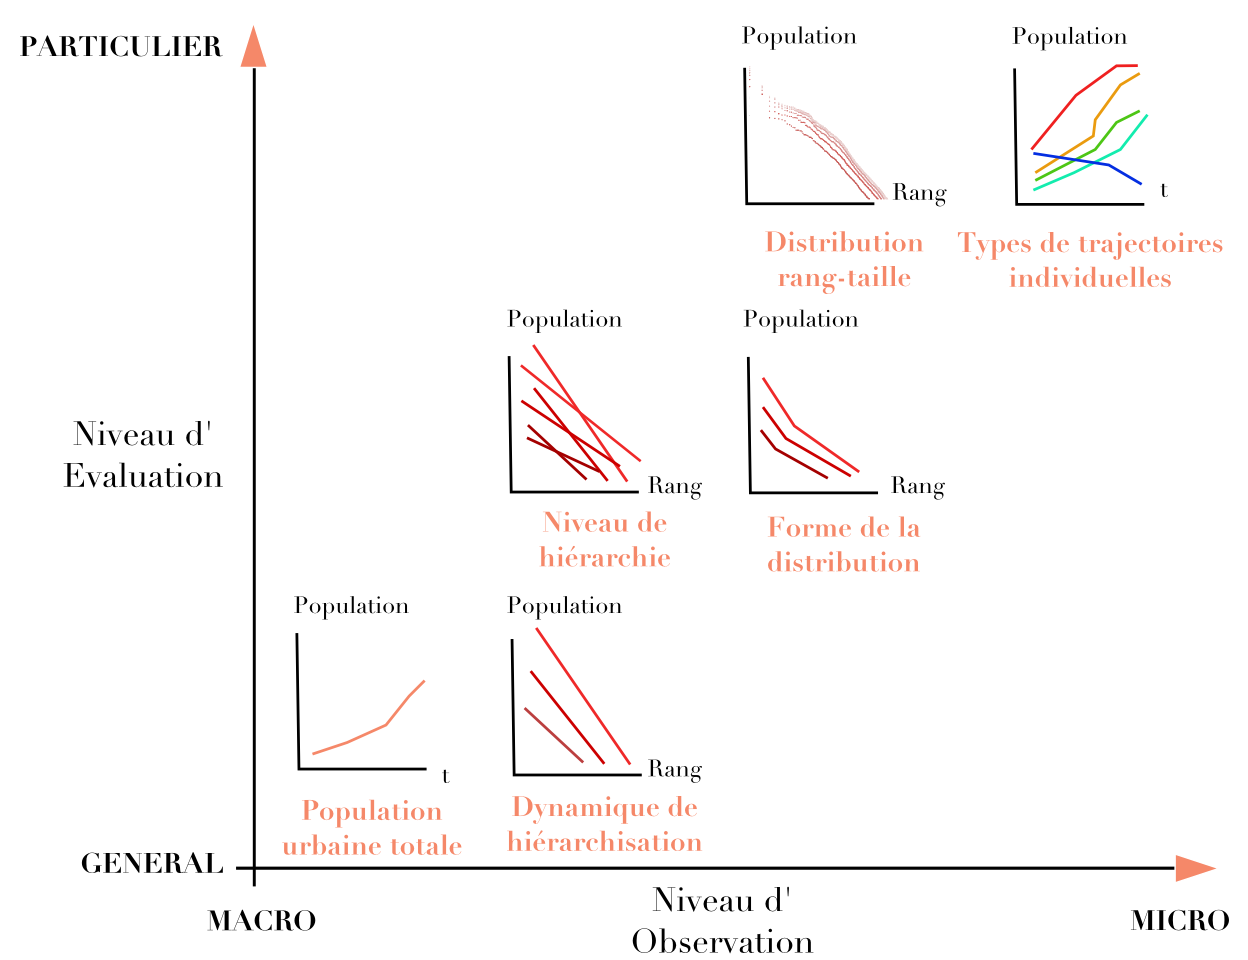
\includegraphics[width=.9\linewidth]{grideval.png}
  \end{sidecaption}
\end{figure}

D'un autre côté, l'activité abductive, même si elle paraît se concentrer initialement sur la construction du modèle de simulation, ne s'applique pas qu'à celui-ci, car le modèle de simulation n'est qu'un rouage de plus mobilisé -pour ses capacités spécifiques- dans une chaîne de traitements, dans une démarche de construction des connaissances plus globale. Les géographes ont su cumuler les avantages spécifiques des outils au fur et à mesure qu'ils ont pu intégrer la discipline. Il faut prendre un certain recul, et voir que la construction d'un modèle de simulation s'insère dans une chaîne de traitements ouverte comptant plusieurs autres modèles, eux aussi potentiellement en construction, et dont l'articulation tient également d'un raisonnement. Dans son analyse sur la place de l'explication en analyse spatiale, \textcite{Sanders2000} voit d'ailleurs plus dans le rapport de l'outil à la démarche adoptée (exploratoire ou hypothético-déductive) une question d'interprétation. \enquote{Ce sont en effet la manière dont l'outil est inséré dans une chaîne de réflexion et de traitement et l'interprétation des informations figurant en entrée et en sortie qui permettent de donner le statut descriptif ou explicatif d'une démarche.} Avant de conclure un peu plus loin à la fin de son analyse \enquote{[...] il n'y a pas de relation simple et fixe, ni entre les niveaux d'observation et la nature des explications, ni entre les outils de l'analyse spatiale et l'explication. La variété des approches permet de diversifier les éclairages sur les phénomènes que l'on cherche à expliquer. Nos démarches en analyse spatiale consistent ainsi davantage à \enquote{éclairer} qu'à \enquote{démontrer} et identifier des jeux de causalités bien stricts.} Selon Lena Sanders, la démarche généralement adoptée en analyse spatiale fait donc figure d'intermédiaire, et les allers retours entre approches exploratoires et approches plus déductives se rapprochent selon elle de cette démarche abductive décrite par Besse.

A travers l'activité de modélisation, c'est donc toute une chaîne de modélisations qui est appelée pour faciliter cette progression du raisonnement vers la résolution de la problématique initialement posée. La découverte au cours de l'exploration du modèle d'une forte dépendance dans l'expression dynamique de certaines hypothèses peut très bien inciter le modélisateur à explorer de nouveau ces données pour questionner l'existence empirique d'une telle corrélation. On peut également déduire de la découverte de nouveaux motifs dans l'exploration d'un jeu de données (permises par exemple par l'utilisation de nouvelles techniques exploratoires) de nouvelles hypothèses dont on va tester les effets dans un modèle de simulation. Par conséquent les expérimentations, qu'elles soient sur un modèle ou sur un autre, sont susceptibles de se répercuter de façon imprévisible sur toute la chaîne de traitements. Comme le précise \textcite[63]{Mathian2014}, \enquote{Les pratiques sont telles dans le domaine du traitement des données géographiques, qu'aucune démarche n'est la suite linéaire d'une série d'étapes. Cest une combinaison de constructions de modèles de différents niveaux (modèle de données, modèle d'analyse spatiale, modèle statistique, représentations visuelles, modèle de simulation).}

Les avantages et les inconvénients de chacun des modèles, et la flexibilité de leurs relations dans ce qui constitue un véritable système de modèles pour \enquote{représenter, et comprendre l'évolution des phénomènes sociaux et environnementaux inscrits dans l'espace} sont très bien encadrés par les écrits des géographes \textcites{Sanders2000, Mathian2014}. On trouve dans la thèse de \textcite{Cottineau2014a, Cottineau2014b} un travail décrivant de façon très précise les inter-relations fructueuses entre une activité de construction de modèles de simulation et d'autres types de modélisations (statistiques, spatiales).

%et renvoie en alternance aux données et aux modèle de données, qui elle même renvoie aux hypothèses et aux implémentations de ces hypothèses, aux indicateurs et à la façon dont on les a construit, etc.

%De nouveau, on constate l'importance du contexte, et l'impossibilité de s'en détacher \autocite{Amblard2006}.

Si les hypothèses et les critères se construisent et se vérifient pour partie dans un espace-temps qui peut s'avérer très différent de celui mobilisé par et pour la seule simulation, est-il possible d'identifier durant la construction d'un modèle de simulation le moment idéal de leurs introductions ? C'est peu probable, et ce n'est pas cette seule conceptualisation en amont de la construction des modèles qui pourra nous en assurer, car cela reviendrait à confondre la dynamique réelle et complexe d'interactions non linéaires entre hypothèses au sein du modèle avec celles que l'on a imaginés et projetées sur le papier. Il faut ainsi garder en mémoire que cette dynamique se soucie assez peu du sens que l'on a bien voulu rattacher aux hypothèses, aux paramètres que l'on introduit, ou que l'on décide d'introduire à un instant $t$ dans nos constructions. Cette conceptualisation en amont reste évidemment un guide important qui permet de formaliser cette expérimentation.

Comme il est relativement difficile de se projetter dans une telle dynamique de construction, on peut essayer d'exemplifier un peu mieux les questions qui peuvent se poser avec l'introduction (ou le retrait) des hypothèses/critères dans les modèles.

On propose la construction d'un modèle de simulation KISS suivant une trajectoire classique de complexification dont la finalité importe peu dans cet exemple. La première implémentation visée est celle d'un modèle \textit{null theories} \textcite{Railsback2012}. Comme son nom l'indique, l'objectif est de commencer au plus tôt la phase de construction/expérimentation avec un modèle de simulation mobilisant le moins d'hypothèses/critères possible. L'objectif de cette construction est double.

Une première opérationnalisation, même minimale, permet de mettre en évidence la dépendance du modèle conceptuel vis-à-vis du modèle implémenté. Il n'est pas problématique d'avoir un modèle conceptuel détaillé dès le départ, au contraire, mais si on décide de réaliser un modèle de simulation, il faut toujours avoir à l'esprit que c'est de l'expérimentation que dépend la progression du raisonnement. Plus vite celle-ci est mise en marche, plus vite on peut entamer cette progression. Cela permet aussi de ne pas minorer l'étape d'implémentation des hypothèses, qui soulève à elle seule des premières divergences avec le modèle conceptuel. La construction d'un premier modèle aux hypothèses minimales permet aussi de connaître le poids interprétatif attribuable à la structure du modèle ainsi mis à nu. Ce qui permet d’observer dans l’évolution du modèle, quel est l’apport exact de chaque nouvelle hypothèse, ou de chaque nouveau critère dans la dynamique exprimée du modèle.

Les hypothèses et les critères mobilisables durant l'activité de modélisation sont tout à la fois des construits qui émergent de cette chaîne de traitements plus globale qui supporte la progression du raisonnement, que des éléments empruntés d'un catalogue plus général, hérité de plusieurs décennies de modélisations en géographie et vérifié de multiples fois par l'empirie (le modèle gravitaire, la loi rang-taille, etc.).

Les hypothèses et les critères mobilisés supportent de façon implicite des valeurs différentes, qui n'apparaissent pas forcément comme évidentes d'un point de vue extérieur. Il est difficile par exemple d'éliminer une hypothèse en fonction de sa seule mise en défaut observés à un instant $t$ dans la construction d'un modèle, d'autant plus lorsque la présence de celle-ci dans le modèle a du sens dans la résolution d'une problématique.

Peut-être n'était-ce simplement pas le moment pour intégrer cette hypothèse au modèle, celui-ci étant encore trop simple ? Peut-être faut-il activer ou implémenter d'autres hypothèses pour que celle-ci puisse se révéler ? Peut-être que le critère devant rendre compte de cette dynamique n'est pas suffisamment adapté ? Peut-être que l'implémentation proposée n'était tout simplement pas la plus pertinente compte tenu de la dynamique déjà existante ? Peut-être que l'entité choisie pour porter l'hypothèse ne se situe pas à la bonne échelle ?  etc.

Inversement une hypothèse ou un critère valable à un instant $t$ ne le sera peut-être plus à un instant $t + 1$. L'explication et la mise en place cohérentes des hypothèses et des critères se fait donc dans ces allers-retours, dans ces multiples essais. La construction d'un modèle de simulation ne semble pas tenir d'un raisonnement linéaire, car les interactions entre le modélisateur et le modèle sont complexes, et opèrent, comme on le perçoit dans toutes ces questions, à de multiples niveaux, parfois de façon simultanée.

\begin{figure}[htbp]
	\begin{sidecaption}[fortoc]{Exemple d'une démarche de construction cumulative}[fig:S_cumulative]
	 \centering
	 \subbottom[Pendant la construction d'un modèle (\textit{building step}) ce sont différentes hypothèses (ici $A$ et $B$) et différentes versions d'hypothèses (ici versions $\{A_1 \dotsc A_n\}$ et versions $\{B_1 \dotsc B_n\}$) qui vont être développées. Si on veut mettre en oeuvre une approche cumulative et mobiliser toute la combinatoire possible entre les différentes versions des hypothèses implémentées durant la construction du modèle, alors il faut considérer la création d'un graphe de dépendances (\textit{graph dependency}). On s'aperçoit alors que certaines version des hypothèses ne sont pas compatibles les unes avec les autres (ex $A_1$ avec $B_2$). Les figures \ref{fig:S_twomeca} et \ref{fig:S_buildmeca} proposent d'instancier cet exemple dans deux familles d'hypothèses régissant les échanges d'innovations entre des villes dans un système de villes.\label{fig:cumulative_a}]{
	 	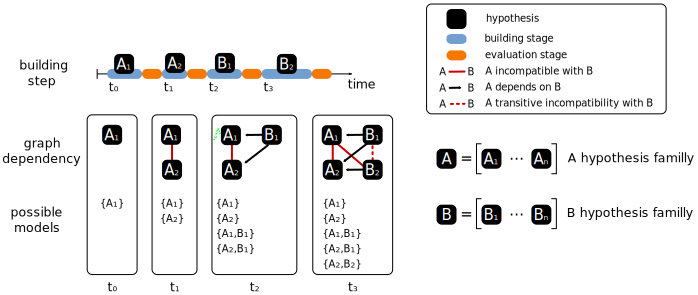
\includegraphics[width=1.0\linewidth]{schema_dependency.pdf}
	 	}\qquad
	 \subbottom[On propose d'étudier plusieurs hypothèses décrivant la façon dont une ville (la ville $i$) peut récupérer et intégrer dans son propre \textit{pool} d'innovations les innovations échangées avec les villes voisines pendant la simulation. Deux niveaux d'hypothèses sont imaginables. Le premier niveau d'hypothèse, le plus simple, propose d'intégrer les innovations à la ville $i$ à chaque fois qu'un échange a lieu avec une autre ville $j$. C'est la famille $A$ dont on trouve deux versions implémentées dans la figure \ref{mechanisme1}. Un deuxième niveau d'hypothèse est envisageable, plus complexe et dépendant du premier niveau il mobilise deux étapes représentées dans la figure \ref{mechanisme2} : 1) on considère l'ensemble des échanges possibles entre la ville $i$ et ses voisines, 2) l'ensemble d'innovations résultant de ces échanges est ensuite filtré puis intégré à la ville $i$ en fonction des règles définies par la famille d'hypothèse $B$ \label{fig:S_twomeca}]{
		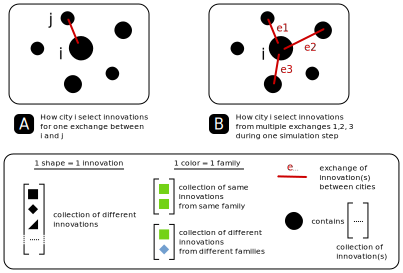
\includegraphics[width=0.8\linewidth]{mechanismslocal.pdf}
		}
	\end{sidecaption}
\end{figure}

\begin{figure}[p]
	\begin{sidecaption}[fortoc]{Présentations des implémentations et des inter-dépendance entre ces implémentations dans le cas des deux familles d'hypothèses $A = \{A_1,A_2\}$ et $B = \{B_1, B_2\}$}[fig:S_buildmeca]
	 \centering
	 \subbottom[Les versions $A_1$ et $A_2$ mobilisent chacune des règles très différentes pour définir là règle de sélection et d'intégration de l'objet innovation échangé entre deux villes $i$ et $j$. La couleur est en effet introduite comme une nouvelle propriété des innovations dans la deuxième version $A_2$ de cette hypothèses $A$.\label{mechanisme1}]{
	 	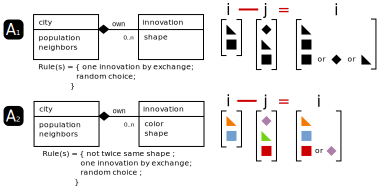
\includegraphics[width=0.9\linewidth]{a1a2mechanism.pdf}
	 	}\qquad
	 \subbottom[Les deux familles de mécanismes sont assemblés en fonction du graphe de dépendance déjà présenté dans la figure \ref{mechanisme1} : $A_1$ est compatible avec $B_1$, mais pas avec $B_2$ car la propriété couleur des innovations est nécessaire à son bon fonctionnement. Les mécanismes $B_1$ et $B_2$ sont par contre tout à fait compatibles avec la version $A_2$. \label{mechanisme2}]{
		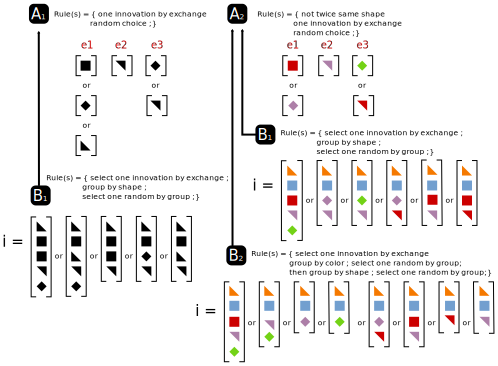
\includegraphics[width=1.0\linewidth]{a1a2b1b2mechanism.pdf}
		}
	\end{sidecaption}
\end{figure}


\begin{figure}[htbp]
\begin{sidecaption}[Evaluation automatique des hypothèses face à des critères multiples]{Les différentes versions des mécanismes sont assemblées dès lors qu'elles sont compatibles (voir le schéma \ref{fig:S_buildmeca}). Les résultats des modèles de simulation ainsi assemblés sont évalués face aux multiples critères experts (qualitatifs, quantitatifs) mobilisés durant la construction. L'hypothèse $A_1$ utilisée à $t_0$ toute seule donne de meilleur résultats que l'hypothèse $A_2$, plus complexe et construite a $t_1$. Il pourrait être tentant d'écarter de suite cette hypothèse, qui reste inférieure à l'hypothèse $A_1$, même une fois couplé à $B_1$ ($\{A_2,B_1\} < \{A_1,B_1\}$). Une fois associée après la phase de construction $t_3$ à la version $B_2$ de l'hypothèse $B$, c'est pourtant la seule combinaison $\{A_2,B_2\}$ qui permettra de satisfaire à la fois le critère 1 et 2.}[fig:S_critererempli]
  \centering
 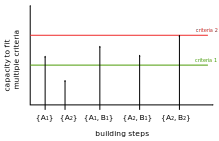
\includegraphics[width=.8\linewidth]{capacity.pdf}
  \end{sidecaption}
\end{figure}

Comme nous nous situons depuis le début dans une problématique de calibrage par optimisation, dont les résultats n'ont pas vocation à être transféré de façon directe à une situation réelle, l'apparition d'un nouveau critère venant contraindre la dynamique peut complétement \enquote{changer la donne} dans cette combinatoire des hypothèses plausibles. Interpréter de telles situations peut rapidement devenir très complexe : 3 hypothèses peuvent produire une dynamique plus proche des critères que 2 hypothèses, mais 1 hypothèse seule peut apparaître meilleure que trois hypothèses sur ce même objectif.

Peut-être que la combinaison de ces deux hypothèses est ici la plus intéressante d'un point de vue des questions thématique qu'elle pose, et cela même si la combinaisons des trois hypothèses produit de meilleurs résultats. Peut être qu'à l'introduction d'un nouveau critère, la solution à deux hypothèses produira des meilleurs résultats, et que l'hypothèse 1 verra ses résultats se dégrader ?

Cette interpretation dépend donc du degré de complexification du modèle au moment où on l'évalue, du nombre de critère retenus pour juger la dynamique de celui-ci, et de la valeur relative que l'on attribue à chacune de ces hypothèses. La figure \ref{fig:S_critererempli} essaye d'exemplifier un tel scénario en s'appuyant sur l'exemple de modèle simplifié présenté dans la figure \ref{fig:S_buildmeca}.

Par conséquent aussi cette possibilité de falsification ou \foreignquote{english}{proof of impossibility}, ne marche que si on est en mesure de prouver l'\textbf{inaptitude constante} d'une d'hypothèse ou d'un jeu d'hypothèses dans la confrontation avec les critères d’évaluation.

Il reste donc à gérer cette possibilité de réengager les hypothèses et les critères à différents moments dans la construction des modèles, et soutenir une activité de construction cumulative (voir la figure \ref{fig:S_cumulative}) qui ne soit pas \enquote{oublieuse} de cette autre espace-temps dans lequel se construisent les hypothèses et les différents critères mobilisés.

